\section{Introduction}

    \subsection{Context/Terminology}

        \begin{frame}[fragile]
            %% João Pizani wants to present this :)
            \frametitle{Source language, Target language}

            \begin{itemize}
                \item Example source code (expression language):
                \begin{verbatim}
Add (Val 1) (Add (Val 1) (Val 3))
                \end{verbatim}

                \item Example target code (for a stack machine):
                \begin{verbatim}
PUSH 1 >> PUSH 1 >> PUSH 3 >> ADD >> ADD
                \end{verbatim}
            \end{itemize}
\end{frame}

    \begin{frame}
        \frametitle{Evaluation, execution}

        \begin{itemize}
            \item An \textbf{eval} function gives the semantics for the \textbf{source} language
                \begin{itemize}
                    \item Denotational semantics
                    \item Maps terms to values
                \end{itemize}

            \item An \textbf{exec} function gives the semantics for the ``\textbf{machine}'' language
                \begin{itemize}
                    \item For each instruction, an operation to perform on the machine state (stack)
                \end{itemize}
        \end{itemize}
    \end{frame}


    \subsection{Compiler correctness}
        \begin{frame}
            %% João Pizani wants to present this :)
            \frametitle{What does "correct" mean?}

            \begin{itemize}
                \item Both semantics (before and after compilation) should be ``equivalent''
                \item Compiling then executing must give the same result as direct evaluation
            \end{itemize}

            \begin{center}
                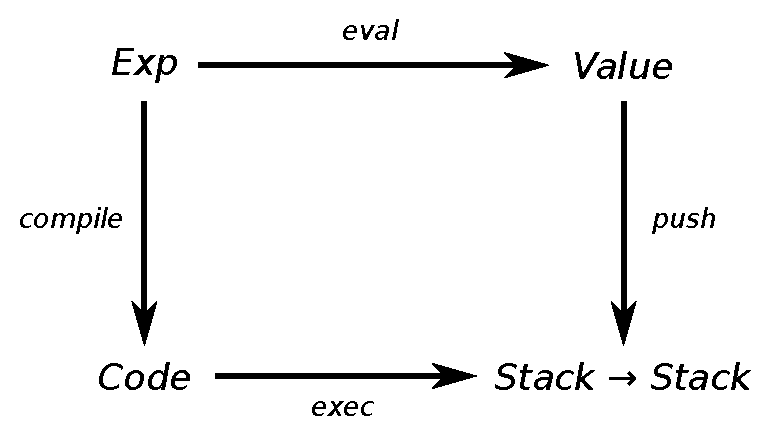
\includegraphics[width=0.75\textwidth]{correctness.pdf}
            \end{center}
        \end{frame}

        \begin{frame}
            %% João Pizani wants to present this :)
            \frametitle{Reference paper}
            \begin{itemize}
                \item "A type-correct, stack-safe, provably correct expression compiler in Epigram"
                    \begin{itemize}
                        \item James McKinna, Joel Wright
                    \end{itemize}

                \item Basic ideas and proofs, which we extended\ldots
            \end{itemize}
        \end{frame}
    

    \subsection{Sharing}
        \begin{frame}[fragile]
            %% João Pizani wants to present this :)
            \frametitle{Extending the source language}

            \begin{itemize}
                \item More "realistic" languages have sharing constructs
                \item We wanted the "simplest possible" extension with sharing behaviour.
                \item \textbf{Chosen extension: if\_then\_else $+$ sequencing}
                    \begin{verbatim}
if c then t else e >> common-suffix
                    \end{verbatim}
            \end{itemize}
            %% Wout draws "diamond" on the board

            \begin{itemize}
                \item The "naïve" compile function will duplicate the suffix
                \item Having Bytecode defined as graph (structured graph) instead of tree
                    would solve this problem
                    \begin{itemize}
                        \item But proofs would be more complex
                    \end{itemize}
            \end{itemize}
\end{frame}


    \subsection{Goals}
        \begin{frame}
            %% Wout presents this? :)
            \frametitle{What we ideally want}

            \begin{itemize}
                \item Have a "smart" graph-based compiler, generating code which uses sharing
                \item Write the correctness proof only for the "dumb" compiler,
                    have correctness \textbf{derived} for the smart version.
              \end{itemize}
        \end{frame}

        \begin{frame}
            %% Wout presents this? :)
            \frametitle{Reference paper}

            \begin{itemize}
                \item "Proving Correctness of Compilers using Structured Graphs"
                    \begin{itemize}
                        \item Patrick Bahr (visiting researcher)
                    \end{itemize}
            \end{itemize}
        \end{frame}

        \begin{frame}
            %% Wout presents this? :)
            \frametitle{Our project's goals}

            \begin{itemize}
                \item Integrating the best of both ``reference'' papers

                \item Our contributions:
                \begin{itemize}
                    \item (Simplest possible) language extension showing sharing behaviour.

                    \item Proof of correctness for the \textbf{stack-safe} ``naïve'' compiler
                        \begin{itemize}
                            \item The one that just duplicates code.
                        \end{itemize}

                    \item A way to to lift this \textbf{stack-safe} "naïve" correctness proof
                        \begin{itemize}
                            \item Into a proof concerning the more \textbf{efficient} compiler.
                        \end{itemize}
                \end{itemize}
            \end{itemize}
        \end{frame}
